\documentclass[../../main.tex]{subfiles}

\begin{document}

Las Redes Neuronales Artificiales (RNAs) son un modelo específico dentro del ML, cuya estructura y funcionamiento están inspirados en el intento de simular los del cerebro. Durante los últimos años, ha sido el área que más desarrollo e impacto ha tenido, principalmente gracias a su versatilidad, potencia y escalabilidad, cualidades que hacen que sean capaces de enfrentar problemas grandes y complejos \cite{hands-on-ML-sklearn-tf}.

% Reseña histórica?
\subsubsection{Breve Contexto Histórico}
Aunque su gran éxito ha sido reciente, lo cierto es que la idea de las RNAs data desde 1943, cuando Warren McCulloch y Walter Pitts presentaron en su artículo \textit{A Logical Caclulus of Ideas Immanent of Nervous Activity} \cite{mculloch-pitts-1943} un modelo computacional simplificado utilizando lógica proposicional acerca de cómo funcionan las neuronas de cerebros animales en conjunto para llevar a cabo cómputos complejos \cite{hands-on-ML-sklearn-tf}. Presentaron una versión muy simplificada de la neurona biológica, que solamente tenía una o más entradas binarias y una salida binaria.

Posteriormente, en 1958, Frank Rosenblatt presentó una de las arquitecturas más simples de RNAs: el ``Perceptrón'' \cite{rosenblatt1958perceptron}, el cual servía principalmente para resolver problemas de clasificación en donde los datos son linealmente separables. Su aporte más notorio es que definió un algoritmo para el entrenamiento del Perceptrón que le permitía mejorar automáticamente sus parámetros internos para poder llegar una solución.

Más tarde, se descubrió que los problemas que no podían ser resueltos por el Perceptrón, sí podían ser resueltos ``apilando'' múltiples perceptrones, lo cual llevó a la invención del ``Perceptrón Multicapa'' (PMC), también conocido como ``Red Neuronal de Propagación Directa'' (del inglés \textit{Feedforward Neural Networks}, FFNN) \cite{deep-learning}. 

Durante los últimos años se han desarrollado diversas \textit{arquitecturas} de redes neuronales, complejizando los algoritmos y las técnicas para lograr resolver determinados tipos de problemas. Sin embargo, todas ellas tienen elementos en común y se entrenan prácticamente de la misma manera. Para explicar estos aspectos, tomaremos como referencia una Red Neuronal Feedforward.

\subsubsection{Red Neuronal Feedforward}


% Función de costo: back-propagation
% Optimizador
% Hiperparámetros: conjunto de validación, cross-validation
% Pesos
% Otras optimizaciones: lotes, detención temprana, dropout

% Neurona Artificial
El elemento básico de cualquier red neuronal es la \textbf{neurona artificial}, que es la que lleva a cabo el ``cómputo''. Una neurona está conectada con otras, de las cuales recibe información y a quienes también les envía. Estas conexiones representan las \textbf{sinapsis} de las neurona biológicas y cada una tiene asociada un determinado número llamado \textbf{peso}, que simboliza la intensidad de la conexión. 

Matemáticamente, lo que hace una neurona es primero computar una suma pesada de sus entradas:
\[z = w_1x_1 + w_2x_2 + \dots + w_nx_n,\]
donde \(x_i\) representa la entrada proveniente de la neurona \(i\) y \(w_i\) es el peso asociado a esta conexión. Esta suma también se puede ver como el producto escalar entre el vector de entradas y el vector de pesos.

Sobre este valor resultante, aplica una \textbf{función de activación} \(h\), siendo como resultado final de la neurona:
\[h(z) = h(w_1x_1 + w_2x_2 + \dots + w_nx_n)\]

Esto se puede ver gráficamente en la Figura \ref{fig:neuron}.

\begin{figure}[h!]
    \centering
    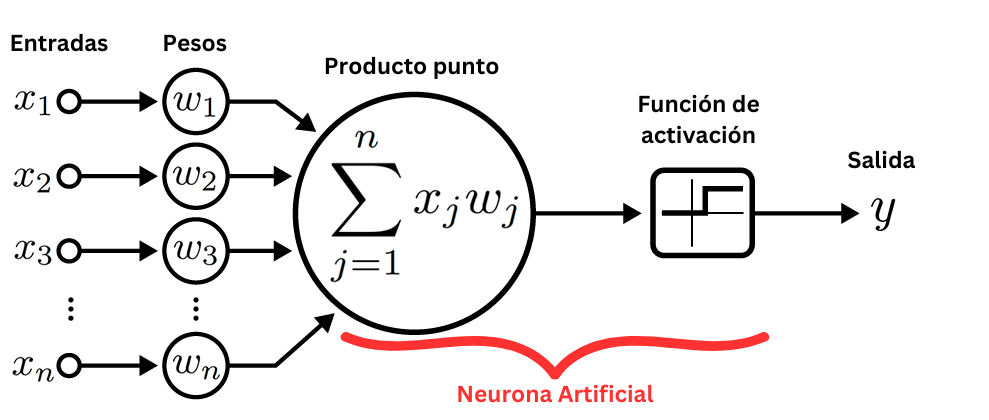
\includegraphics[width=0.6\textwidth]{figs/neurona.png}
    \caption{La neurona computa una suma pesada de sus entradas y aplica una función de activación sobre el resultado.}
    \label{fig:neuron}
\end{figure}

La idea detrás de la función de activación es el hecho de propagar la información proporcionalmente al estímulo provocado por las entradas en la neurona, basándose en la idea de ``disparo'' de una neurona biológica en el momento en que se supera el umbral de activación. La función de activación utilizada en el Perceptrón, mencionado anteriormente, fue la llamada \textit{heavyside}, dada por:
\[
    heavyside\left(z\right) =
        \begin{cases}  
            0\text{ si }z < 0 \\
            1\text{ si }z \geq 0
        \end{cases}
\] 

Durante los años, se han empleado diferentes funciones de activación, como la sigmoide, la tangente hiperbólica, y la ReLU, dada por \(\text{ReLU}(z)=\text{max}(0, z)\), siendo esta última la más común actualmente.

Dicho esto, en una red neuronal está compuesta por diferentes \textbf{capas de neuronas}: la capa de entrada, que es por donde ingresan los datos, una o más capas ocultas o intermedias, y finalmente la capa de salida. 

En una red Feedforward particularmente, las neuronas de una capa están conectadas solamente con las neuronas de la capa siguiente, implicando de esta forma que la información fluye solamente en una dirección (de aquí la nomenclatura Feedforward). Algo a notar también sobre estas redes es que cada neurona de una capa está conectada con todas las neuronas de la capa siguiente, razón por la cual este tipo de conexión también se suele llamar ``densa''. Esta situación puede verse en la Figura \ref{fig:neural-net}. 

\begin{figure}[h!]
    \centering
    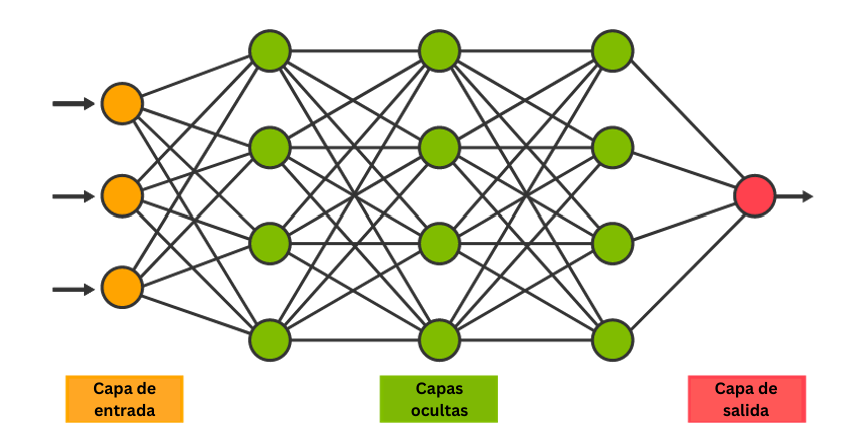
\includegraphics[width=0.6\textwidth]{figs/feedforward.png}
    \caption{Esquema de una Red Neuronal Profunda, con tres capas ocultas. Las neuronas naranjas forman la capa de entrada, las neuronas verdes forman las tres capas ocultas, y la roja la de salida. Cabe notar que la capa de salida podría tener más de una neurona.}
    \label{fig:neural-net}
\end{figure}

Ahora bien, el objetivo de una red neuronal es \textbf{aproximar una función desconocida} \(g^*\). Para un clasificador por ejemplo, \(y=g^*(x)\) determina una categoría \(y\) para una entrada \(x\). De esta forma, una red define una asignación \(y=g(x; \theta)\) y aprende el valor de los \textbf{parámetros} \(\theta\) que resultan en la mejor aproximación de la función ``oculta'' \cite{deep-learning}. En este caso, los parámetros a aprender por la red serán los pesos sinápticos de todas las conexiones.

Matemáticamente, los pesos entre una capa de neuronas y la siguiente se pueden pensar como una matriz \(w\), en donde la entrada \(w_{ij}\) indica el peso sináptico de la conexión entre la neurona \(i\) de la capa ``actual'' y la neurona \(j\) de la capa ``anterior''. La pregunta que surge entonces es \textbf{cómo} hacer para que la red pueda aproximar esta función.

\subsubsection{Entrenamiento de una RNA Feedforward}
A grandes rasgos, el entrenamiento de una red consiste en una suma de \textbf{evaluación} y \textbf{optimización} \cite{pedro-domingos}. Con evaluación, nos referimos al establecimiento de una medida que determine qué tan lejos está el modelo de hallar una buena solución, para lo cual se suele definir una función a minimizar o maximizar llamada \textbf{función objetivo} o \textbf{criterio} \cite{deep-learning}; y la optimización es el método usado para aproximarse a dicha solución, maximizando o minimizando la función objetivo según corresponda.

Cuando lo deseado es minimizar la función objetivo, esta pasa a ser llamada \textbf{función de costo}, \textbf{función de error} o \textbf{función de pérdida}. En problemas de aprendizaje supervisado, esta función compara la salida de la red para determinadas entradas - la \textbf{predicción} - en su estado actual, dado por el valor de los pesos sinápticos en ese momento, con las salidas reales para dichas entradas, dadas por el conjunto de entrenamiento. En resumen, una vez que están fijos los datos del conjunto de entrenamiento, la función de costo es una función de los pesos de la red. Por lo tanto, la denotaremos con \(f(w)\).

Dos de las funciones de costo más utilizadas son el \textbf{Error Cuadrático Medio} y la \textbf{Entropía Cruzada}. De estas dos funciones, nos concentraremos en la última ya que es la más apropiada para problemas de clasificación como el que tratamos. Esto se debe a que mide la diferencia entre la distribución de probabilidad predicha por el modelo y la distribución real de los datos.  En este caso, la capa de salida tiene tantas neuronas como categorías haya, y la salida de cada una de ellas representa el puntaje que le da la red a la categoría correspondiente a cada neurona, donde un mayor puntaje indica una mayor probabilidad de pertenencia de la entrada particular a dicha clase. Para obtener una estimación de la distribución de probabilidad dada por estas salidas, se aplica la función \textit{softmax} \cite{hands-on-ML-sklearn-tf}.

Una vez que se tiene esta función establecida y se calculan las pérdidas para los datos, el algoritmo por defecto que se utiliza para la optimización es el de \textbf{Descenso por el Gradiente} (\textit{Gradient Descent}). Este se basa en modificar los parámetros (i.e. los pesos sinápticos) iterativamente con el objetivo de encontrar mínimos locales de una función, que en este caso será la de costo. Se basa en la idea que la dirección dada por el gradiente es la de mayor crecimiento, y por lo tanto su opuesta es la de menor. De esta forma, lo que se hace en cada paso es calcular el gradiente de la función de costo con respecto a los pesos, y luego actualizarlos siguiendo la siguiente regla:
\[
w = w - \eta \ \nabla f(w),
\]
donde \(w\) representa una matriz de pesos de una determinada capa, y la cantidad \(\eta\) es llamada la \textbf{tasa de aprendizaje}, que determina el tamaño de cada paso. Si \(\eta\) es muy pequeño, entonces el algoritmo tendrá que hacer muchos pasos para converger; pero si es demasiado grande, puede llegar a divergir. 

Actualmente, se utilizan otros optimizadores más sofisticados y eficientes, pero que todos parten de la idea del Descenso por el Gradiente. Los que usaremos en los experimentos son el Descenso por el Gradiente Estocástico (\textit{Stochastic Gradient Descent}, SGD) y Adam (\textit{Adaptive Moment Estimation}), de los cuales se puede leer más en el Capítulo 8 de \cite{deep-learning}.

Ahora bien, recordando que la función \(f\) está fija en todas las entradas y salidas del conjunto de entrenamiento, hay algoritmos de optimización que utilizan todos estos datos para  calcular el gradiente, otros que utilizan de a un ejemplo a la vez para calcular el gradiente y otros que están entre medio de los dos anteriores, es decir utilizan un subconjunto del conjunto de datos para calcular el gradiente (esto es lo que hace SGD). 

Es necesario en este punto introducir el concepto de ``\textbf{época}'' y de ``\textbf{lote}''. Un lote es simplemente una subdivisión de tamaño fijo del conjunto de entrenamiento (o de test). Dicho esto, se llama época al proceso completo en el cual el modelo entrena utilizando \textbf{todos} los datos disponibles en el conjunto de entrenamiento una vez, ya sea recorriéndolos de a lotes o todos de una vez. Si el conjunto está efectivamente dividido en lotes, una época va a consistir de: \textbf{para cada lote}, calcular las predicciones en base a los pesos actuales, obtener los errores de cada muestra del lote, computar los gradientes en base a los ejemplos del lote y actualizar los pesos. Si no, se hacen los mismos pasos pero para todos los datos de una vez.

Al entrenar un modelo, existen ciertos ajustes que son utilizados para controlar su comportamiento llamados \textbf{hiperparámetros}. Los valores de los hiperparámetros no son aprendidos por el modelo \cite{deep-learning}, sino que se fijan de antemano y no se modifican a lo largo del entrenamiento. Algunos de estos son: la cantidad de neuronas en cada capa oculta, la función de activación utilizada en cada capa, el optimizador, la tasa de aprendizaje, el número de épocas, el tamaño de lote, entre otros. Todos estos pueden contribuir a que el modelo mejore su desempeño. Para probar distintos valores de hiperparámetros, que es lo que haremos a continuación, se utiliza un conjunto de datos extra además del de entrenamiento y el de test, llamado de \textbf{validación} que sirve justamente para encontrar los hiperparámetros óptimos.

% Mejoras extras: detención temprana, dropout
Otras mejoras que se han implementado para mejorar la eficacia de los modelos, y que emplearemos en los experimentos, son las nombradas a continuación. Por un lado, tenemos la \textbf{detención temprana}, que consiste en frenar el entrenamiento en el último mejor ``estado'' del modelo cuando se observa que a partir de dicho punto el error sobre el conjunto de validación no mejora (notar que cuántas épocas se espera y qué se considera una mejora son nuevos hiperparámetros). Y por otro lado, el \textbf{dropout}, que es un algoritmo que implica suprimir un cierto número de neuronas de una capa de manera aleatoria \cite{apuntes-redes-neuronales}. 

\end{document}